\documentclass[sigconf,review,anonymous]{acmart}

\usepackage{booktabs} % For formal tables

% Copyright
\setcopyright{none}
%\setcopyright{acmcopyright}
%\setcopyright{acmlicensed}
%\setcopyright{rightsretained}
%\setcopyright{usgov}
%\setcopyright{usgovmixed}
%\setcopyright{cagov}
%\setcopyright{cagovmixed}


% DOI
\acmDOI{10.475/123_4}

% ISBN
\acmISBN{123-4567-24-567/17/06}

%Conference
\acmConference[SIGGRAPH 2017 Posters]{SIGGRAPH 2017 Posters}{August 2017}{Los Angeles, CA, USA} 
\acmYear{2017}
\copyrightyear{2017}
\acmPrice{15.00}

% use the "authoryear" citation style.
\citestyle{acmauthoryear}
\setcitestyle{square}

\begin{document}
\title{GRNsight: a web application and service for visualizing models of small- to medium-scale gene regulatory networks}

\author{Eileen Choe}
\orcid{1234-5678-9012}
\affiliation{%
  \institution{Loyola Marymount University}
  \streetaddress{1 LMU Drive}
  \city{Los Angeles} 
  \state{California} 
  \postcode{43017-6221}
}
\email{trovato@corporation.com}

\author{G.K.M. Tobin}
\affiliation{%
  \institution{Institute for Clarity in Documentation}
  \streetaddress{P.O. Box 1212}
  \city{Dublin} 
  \state{Ohio} 
  \postcode{43017-6221}
}
\email{webmaster@marysville-ohio.com}

% The default list of authors is too long for headers}
\renewcommand{\shortauthors}{B. Trovato et. al.}

\begin{abstract}

We present new visualization and display features in v2 of GRNsight, a web application and service optimized for visualizing small- to medium-scale gene regulatory networks (GRNs). A GRN consists of genes, transcription factors, and the regulatory connections between them which govern the level of expression of mRNA and protein from genes. GRNsight produces weighted or unweighted network graphs from an Excel spreadsheet containing an adjacency matrix where regulators are named in the columns and target genes in the rows, a Simple Interaction Format (SIF) text file, or a GraphML XML file. GRNsight represents genes as nodes and regulatory connections as edges with colors, end markers, and thicknesses corresponding to the sign and magnitude of activation or repression. GRNsight visualizations can be modified through manually dragging nodes or adjusting sliders that change the force graph parameters. GRNsight is best-suited for visualizing networks of fewer than 35 nodes and 70 edges, and has general applicability for displaying any small, unweighted or weighted network with directed edges for systems biology or other application domains. The GRNsight application (http://dondi.github.io/GRNsight/) and code (https://github.com/dondi/GRNsight) are available under the open source BSD license.

\end{abstract}

%
% The code below should be generated by the tool at
% http://dl.acm.org/ccs.cfm
% Please copy and paste the code instead of the example below. 
%
\begin{CCSXML}
<ccs2012>
<concept>
<concept_id>10003120.10003145.10003147.10010364</concept_id>
<concept_desc>Human-centered computing~Scientific visualization</concept_desc>
<concept_significance>500</concept_significance>
</concept>
<concept>
<concept_id>10003120.10003145.10003151.10011771</concept_id>
<concept_desc>Human-centered computing~Visualization toolkits</concept_desc>
<concept_significance>500</concept_significance>
</concept>
</ccs2012>
\end{CCSXML}

\ccsdesc[500]{Human-centered computing~Scientific visualization}
\ccsdesc[500]{Human-centered computing~Visualization toolkits}

% We no longer use \terms command
%\terms{Theory}

\keywords{Scientific Visualization, Software Engineering, Bioinformatics}

\begin{teaserfigure}
  \centering
  %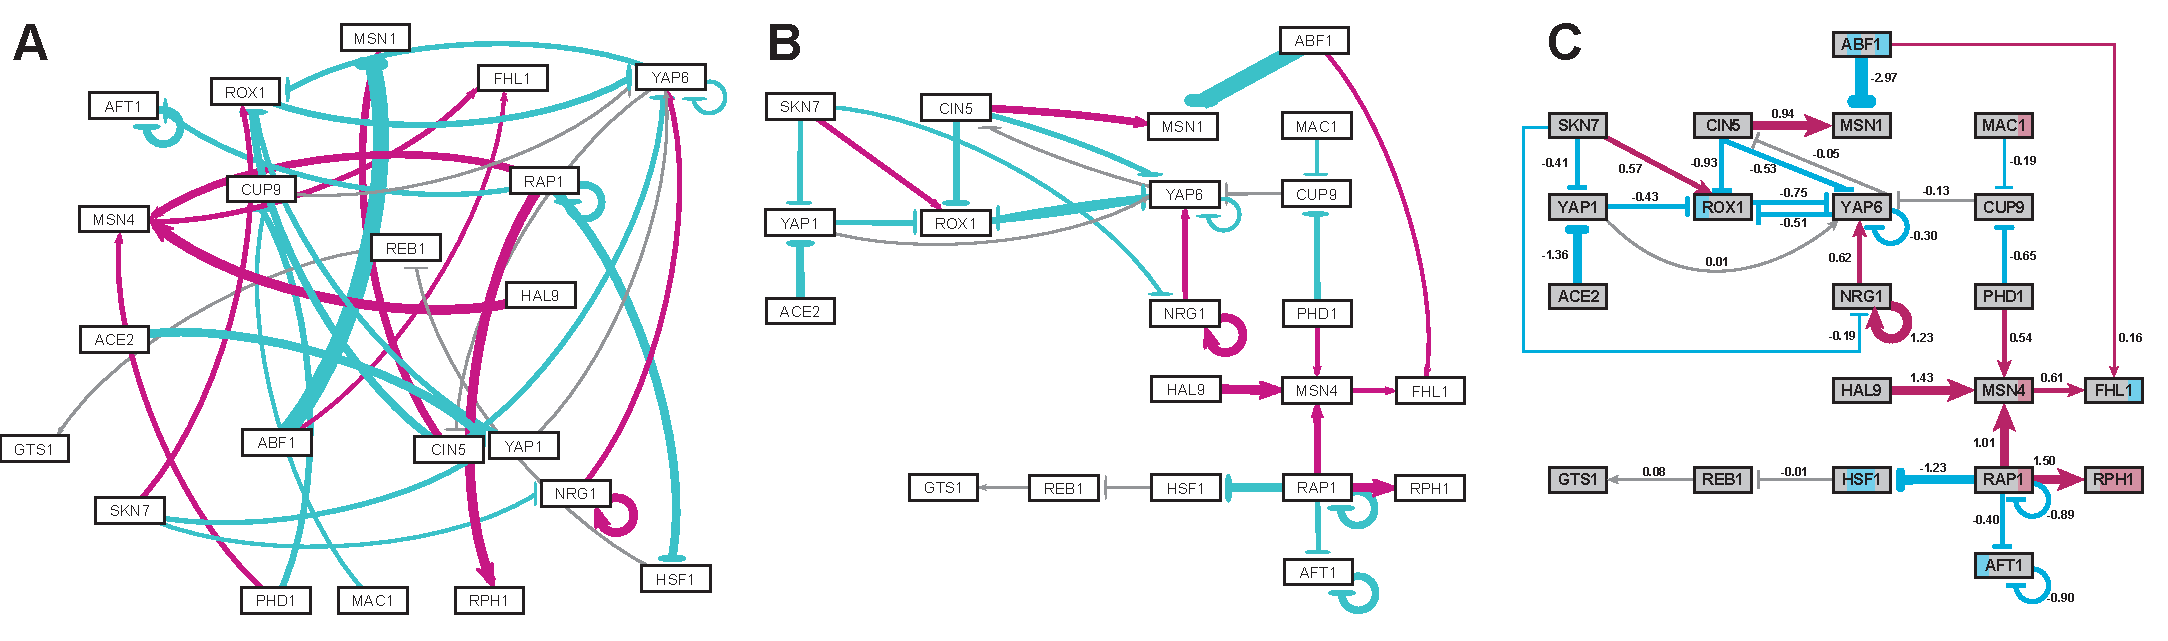
\includegraphics[width=\textwidth]{comparison.pdf}
  \includegraphics[height=2in]{screenshot-always-show-weights.png}
  \caption{Screenshot of GRNsight.}
  \label{fig:teaser}
\end{teaserfigure}


\maketitle

\section{Introduction and Motivation}

GRNsight is a web application and service for visualizing models of small- to medium-scale gene regulatory networks (GRNs) that is optimized for use by novice and experienced biologists alike to quickly and easily view unweighted and weighted network graphs. Visual inspection has long been recognized as distinct from other forms of purely numeric, computational, or algorithmic data analysis \cite{mulrow2002visual, card1999readings}, and GRNsight enables the potential for insight derived specifically by visual inspection. The following are the requirements for GRNsight:

\begin{enumerate}
\item Exist as a web application without the need to download and install specialized software;
\item Be simple and intuitive to use;
\item Automatically lay out and display small- to medium-scale, unweighted and weighted, directed network graphs in a way that is familiar to biologists and adds value to the interpretation of the modeling results.
\end{enumerate}


\noindent\textbf{Graph Customizations and User Interface}: GRNsight's diagrams are based on force graph layout algorithms in the D3.js visualization library \cite{d3}, which was then extensively customized to support the specific needs of biologists for GRN visualization. The GRNsight user interface includes a menu/status bar and sliders that adjust D3.js's force graph layout parameters, to refine the automated visualization. Design decisions for the user interface were driven by applicable interaction design guidelines and principles \cite{norman2013design,shneiderman2010designing,nielsen1994usability} in alignment with the mental model and expectations of the target user base, consisting primarily of biologists.\\

\noindent\textbf{Data Interoperability}: GRNsight supports Excel spreadsheet, a Simple Interaction Format (SIF) text file, or a GraphML XML file, and can export networks to Simple Interaction Format (SIF) text file, or a GraphML XML file...\\

\noindent
Since the release of GRNsight v1, further study on effective visualization techniques as well as feature requests from peer review have motivated the following improvements to GRNsight in v2.

\section{Extensions to GRNsight in v2}

\subsection{Separation of Viewport from Graph Bounding Box}
Problem: Allow graph to relax
Solution: The bounding box and viewport for the graph have been separated allowing for the following new features: 
- The bounding box can now be fixed to the size of the viewport or adapted to the size of the graph
- The viewport size can be selected from among small, medium, and large options
- The best viewport size is automatically detected from the browser
- The viewport can be fit to the size of the browser window 
- Zooming and scrolling have been enabled


\subsection{Edge Weight Display Options}
When a weighted graph is loaded, the user now has the options to show weights upon mouseover of an edge, always show weights, or never show weights

\subsection{Graph Normalization}
The user can set the maximum and minimum values to which the edge thicknesses are normalized in a weighted graph

\subsection{Improvements to Visualization}
- Reducing the white space on either side of a node label for long labels
- Setting the minimum size of a node
- Making the pointed arrowhead larger for the thinnest edges
- Improving the appearance of self-regulatory edges for nodes with long labels
- Minor adjustments to the placement and centering of edge end-markers

\subsection{"Under the Hood"}
- The versions of package dependencies have been standardized and documented in the package.json file
- Code has been ported to version v0.7.2 of Node-xlsx
- Testing suite has been refactored into semantic and syntactic tests
- Additional syntactic tests have been written for SIF and GraphML formats
- A cap has been placed on the number of errors returned according to a tunable strictness parameter 

\section{Conclusion and Future Work}
We have successfully implemented GRNsight, a web application and service for visualizing small- to medium-scale GRNs that is simple and intuitive to use. GRNsight accepts an input file, reading reading a weighted or unweighted representation of a GRN, and automatically lays out and displays unweighted and weighted network graphs, enabling interpretation of the weight parameters more easily than one could from the adjacency matrix alone. Extensions to GRNsight in v2 have improved GRNsight's ...

Future work...

\bibliographystyle{ACM-Reference-Format}
\bibliography{siggraph-abstract-review} 

\end{document}
